\documentclass[../psets.tex]{subfiles}

\pagestyle{main}
\renewcommand{\leftmark}{Problem Set \thesection}

\begin{document}




\section{Applications of Molecular Orbitals}
\marginnote{9/25:}The questions pertain to the material we have covered from Introduction (Sep 5) to Pericyclic Reactions (Sep 19). For the molecular orbital (MO) diagrams, please draw the MOs with appropriate energy levels, fill in the electrons, and draw cartoons that illustrate the orbital
interactions.
\begin{enumerate}
    \item The geometry of \ce{PMe3} (\textbf{1}) is known to be pyramidal.
    \begin{center}
        \includegraphics[width=0.12\linewidth]{PSet1F1.png}\\
        \textbf{1}
    \end{center}
    A qualitative MO diagram for the frontier orbitals of \ce{PMe3} can be drawn as follows.
    \begin{center}
        \includegraphics[width=0.4\linewidth]{PSet1F2.png}
    \end{center}
    \begin{enumerate}
        \item How will the energies of the frontier orbitals change if we decrease one \ce{C-P-C} angle, denoted as $\theta$, by symmetrically moving the two methyl groups closer to each other? Draw a Walsh diagram for the frontier orbitals to explain. Assume that the bond lengths are unchanged.
        \begin{proof}
            Let's consider the energy changes orbital by orbital, from bottom to top.\par
            \begin{center}
                \includegraphics[width=0.9\linewidth]{PSet1Q1a.png}
            \end{center}
            \underline{HOMO}: As $\theta$ decreases with fixed bond lengths, the two methyl orbitals adjacent to $\theta$ get closer and begin to participate in a \emph{slightly} stabilizing, secondary interaction. This will cause the HOMO to go down in energy slightly.\par
            \underline{Bottom LUMO}: As $\theta$ decreases, we will observe the same slightly stabilizing secondary interaction as in the HOMO. However, this effect will be dwarfed with increasing primary destructive interference with the phosphorous atom's shaded $p$-lobe. Thus, the energy of this orbital will go up more than the energy of the HOMO went down.\par
            \underline{Top LUMO}: As $\theta$ decreases, we'll gain some destructive secondary interference, but we'll mostly lose primary destructive interference as we approach a primary nonbonding orientation in the nodal plane of the $p$-orbital. Thus, the energy of this orbital will go down on a similar order of magnitude to how much the bottom LUMO went up.
        \end{proof}
        \item How will the energies of the frontier orbitals change if we instead increase $\theta$ while maintaining the bond lengths? Draw a Walsh diagram for the frontier orbitals to explain.
        \begin{proof}
            Similarly to part (a), we will also do this analysis orbital by orbital, from bottom to top.\par
            \begin{center}
                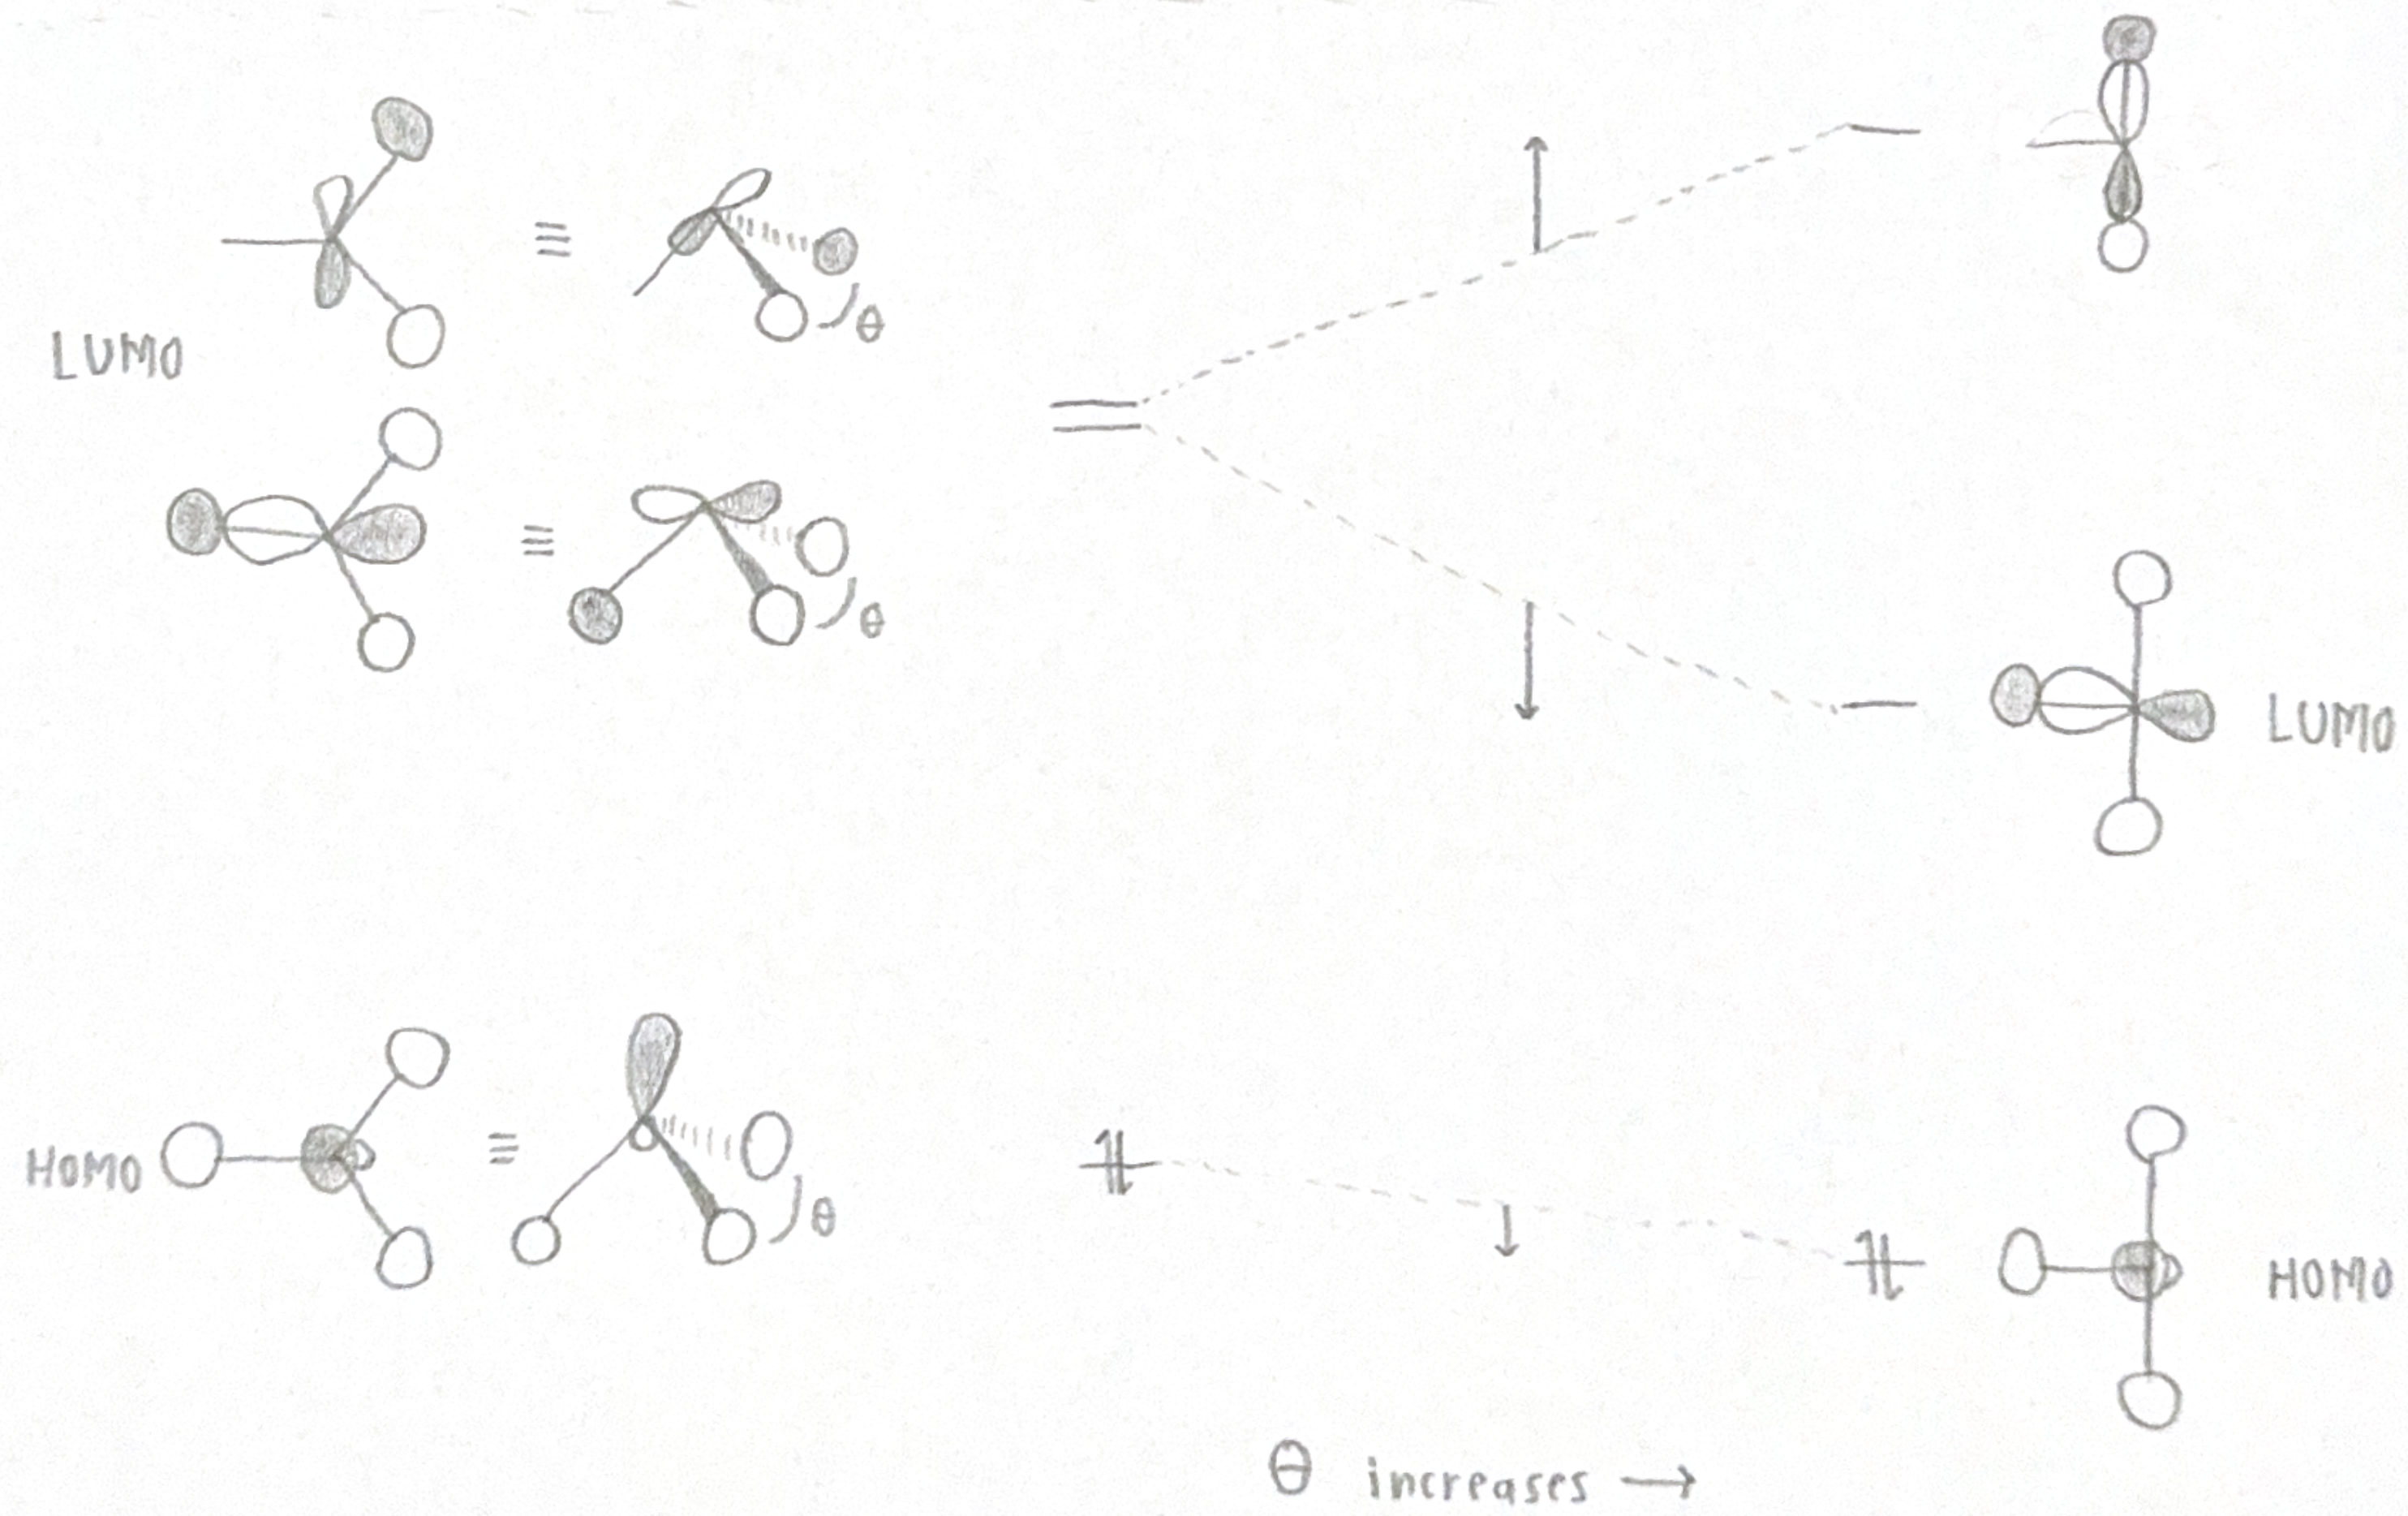
\includegraphics[width=0.9\linewidth]{PSet1Q1b.png}
            \end{center}
            \underline{HOMO}: As $\theta$ increases with fixed bond lengths, the two methyl orbitals adjacent to $\theta$ \emph{both} get closer to the methyl on the left side of the diagram. This will induce another \emph{slightly} stabilizing, secondary interaction, but likely a slightly bigger stabilizing interaction than the analogous one in part (a).\par
            \underline{Bottom LUMO}: Decreasing primary destructive interference between the shaded $p$-lobe and the two unshaded methyl lobes that are moving results in a net stabilizing interaction that is more significant than the slightly stabilizing interaction in the HOMO.\par
            \underline{Top HOMO}: Increasing primary destructive interference leads to a similarly significant destabilizing interaction.
        \end{proof}
        \item Rank the relative nucleophilicity and electrophilicity of the following molecules, and rationalize your hypotheses.
        \begin{center}
            \includegraphics[width=0.5\linewidth]{PSet1F3.png}
        \end{center}
        \begin{proof}
            $\theta$ is unstrained in \textbf{4}, $\theta$ is slightly decreased in \textbf{3}, and $\theta$ is more decreased in \textbf{2}. Additionally, a higher energy/more destabilized HOMO will make a species more nucleophilic, and a lower energy/more stabilized LUMO will make a species more electrophilic. Thus, all we need to answer this question is the MO diagram in part (a).\par
            Since the HOMO gets more stabilized as $\theta$ decreases,
            \begin{center}
                \fbox{\textbf{4} is the most nucleophilic, then \textbf{3}, then \textbf{2}.}
            \end{center}
            Since the LUMO also gets more stabilized as $\theta$ decreases,
            \begin{center}
                \fbox{\textbf{2} is the most electrophilic, then \textbf{3}, then \textbf{4}.}
            \end{center}
        \end{proof}
    \end{enumerate}
    \item Consider the combination of two allyl fragments (\textbf{1}) joined at the center carbons, leading to diradical (\textbf{2}).
    \begin{center}
        \includegraphics[width=0.35\linewidth]{PSet1F4.png}
    \end{center}
    \begin{enumerate}
        \item Construct a $\pi$ MO interaction diagram for \textbf{2} that predicts the symmetries of the combined MOs and their energies relative to carbon $p$-orbitals. Please assume that only interactions between AOs on \underline{adjacent atoms} are significant.
        \begin{proof}
            {\color{white}hi}
            \begin{center}
                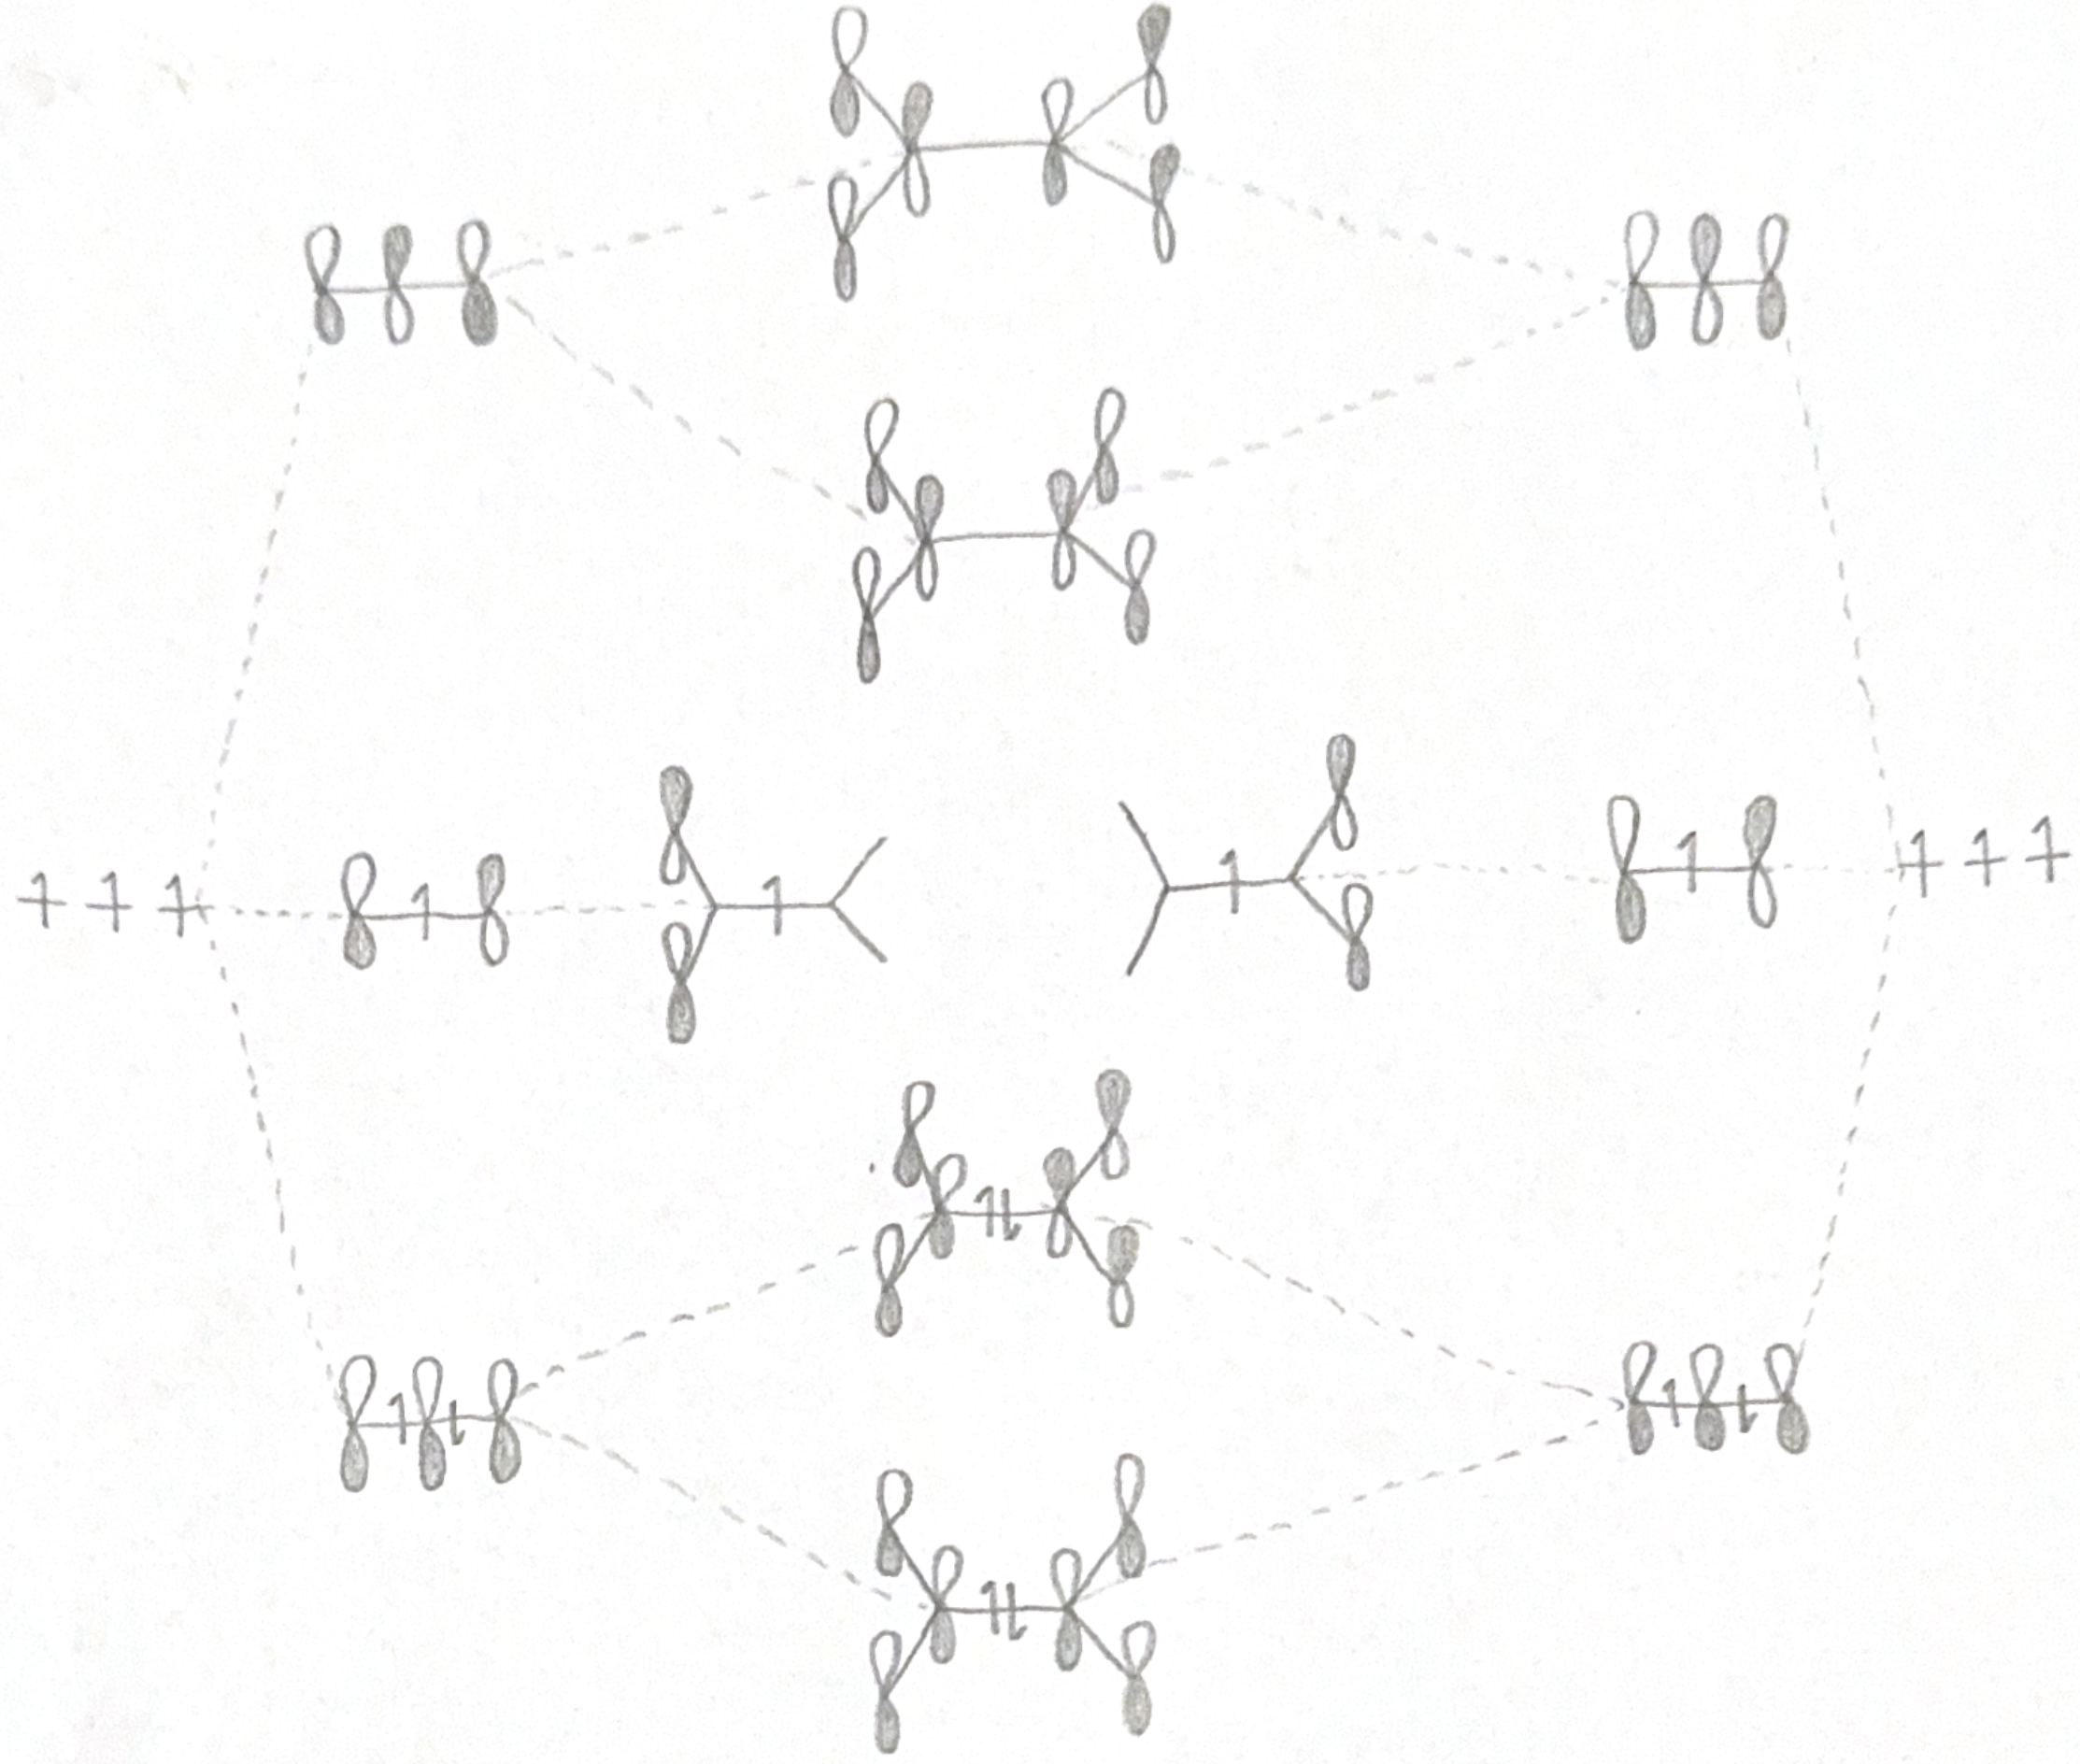
\includegraphics[width=0.9\linewidth]{PSet1Q2a.png}
            \end{center}
            Since this MO diagram only considers $\pi$-orbitals, we begin by drawing two sets of standard allyl MOs that we will subsequently mix. Each set of allyl MOs is composed of three $p$-orbitals. Additionally, since there are 2 $\pi$-electrons in the double bond and 1 $\pi$-electron in the radical, each set of $\pi$-MOs is occupied by three electrons.\par
            As we begin mixing, we only mix MOs of similar energies. In this case, that means we only mix MOs directly across. Note that we do \emph{not} mix the middle MOs because the problem statement tells us that only MOs with "adjacent atom" interactions should mix, and these MOs have no electron density in the center where the $\sigma$-bond forms. Additionally, note that we only have electron density on one side or the other (rather than both) because if we had it on both, that would imply that we are adding or subtracting wavefunctions; in other words, the mixed orbitals are of the form $\psi_1\pm\psi_2$ and the degenerate orbitals are of the form $\psi_1,\psi_2$.
        \end{proof}
        \item Can the two radical centers delocalize via resonance? Explain using the MO diagram from part (a).
        \begin{proof}
            \fbox{No.} Per the MO diagram, we still have a diradical in the HOMO, and each radical electron is localized in an MO on one side of the molecule.
        \end{proof}
    \end{enumerate}
    \item Predict the stereochemistry of the product and rationalize your answer based upon MO theory.
    \begin{center}
        \includegraphics[width=0.5\linewidth]{PSet1F5.png}
    \end{center}
    \begin{proof}
        {\color{white}hi}
        \begin{center}
            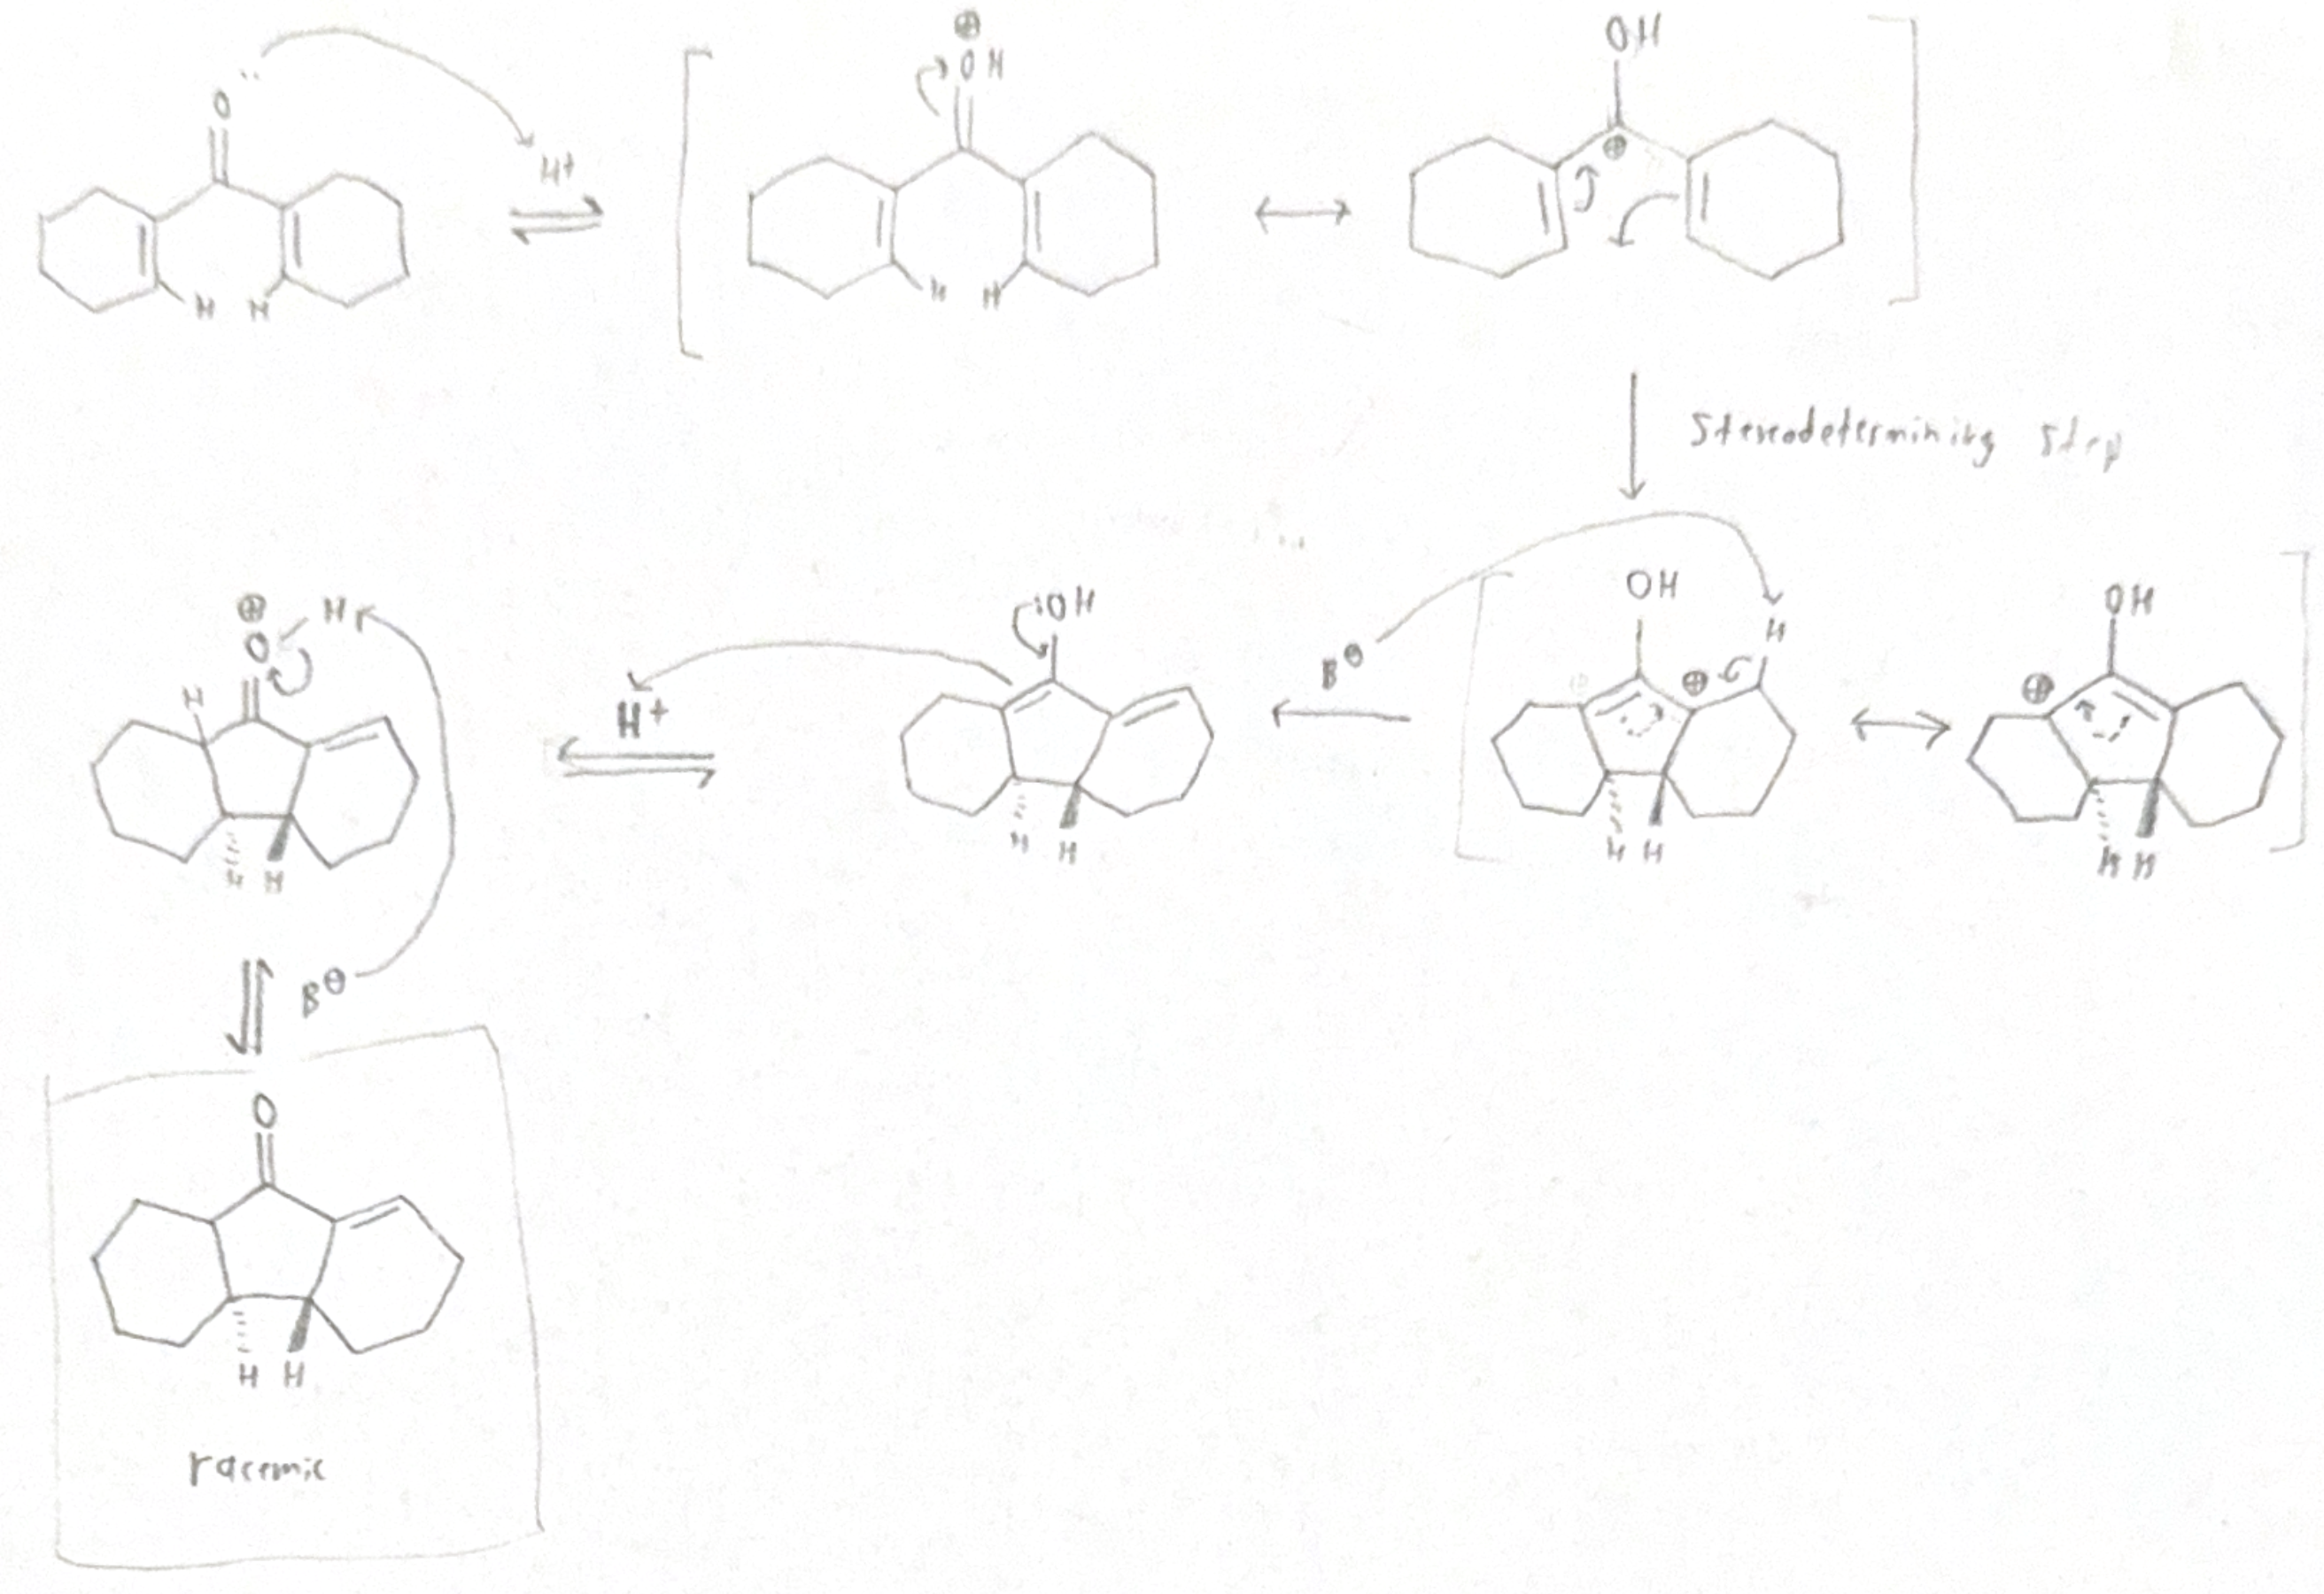
\includegraphics[width=0.9\linewidth]{PSet1Q3-1.png}
        \end{center}
        The stereodetermining step is a cationic $4\pi$ electrocyclization, more commonly known as a \textbf{Nazarov cyclization}. Note that a few steps are necessary before the cyclization to activate the substrate, and a few are necessary afterwards to convert to the final product.
        \begin{center}
            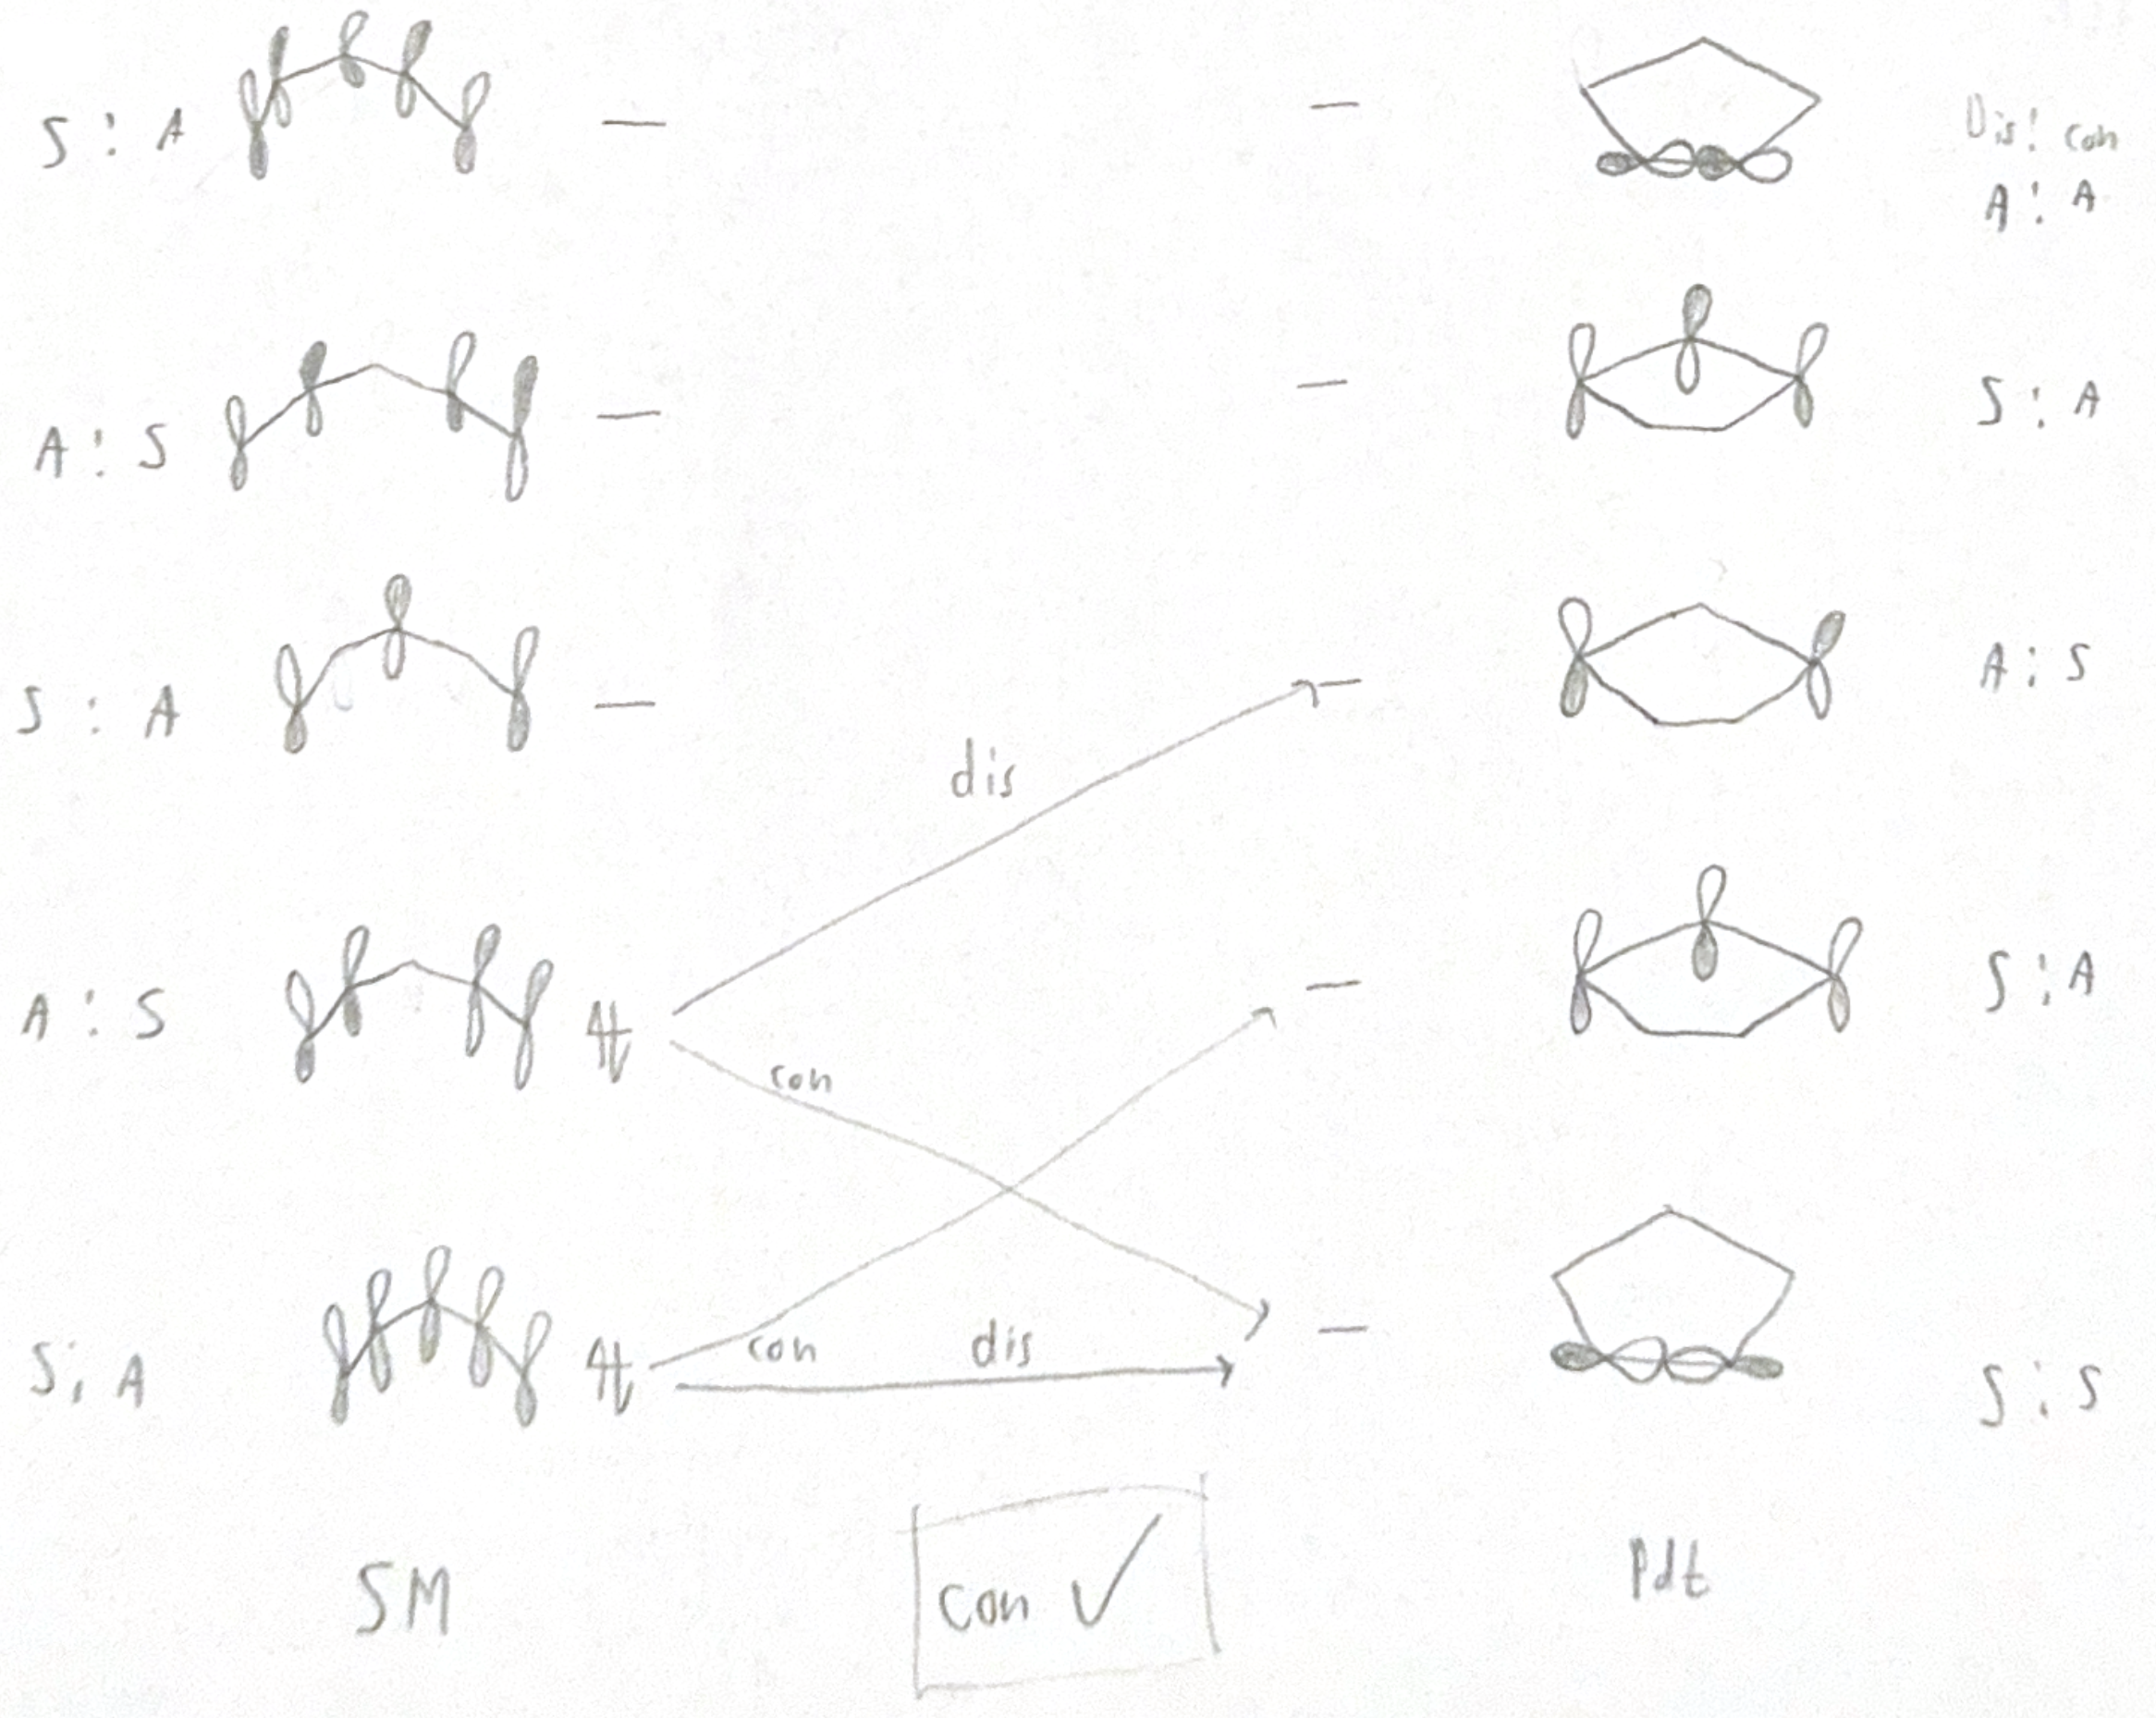
\includegraphics[width=0.9\linewidth]{PSet1Q3-2.png}
        \end{center}
        The reason that the electrocyclization occurs in a conrotatory fashion is that the thermal symmetry-allowed transitions do not move electrons up in energy levels, whereas the thermal symmetry-allowed disrotatory transitions do and hence are disfavored. Note that I did not show the \ce{R} groups for simplicity.\par
        Additional notes: This problem can also be solved using FMO and rotation.
    \end{proof}
    \item Norbornadiene is known to be more reactive towards electrophiles than norbornene.
    \begin{center}
        \includegraphics[width=0.37\linewidth]{PSet1F6.png}
    \end{center}
    \begin{enumerate}
        \item Rationalize this difference using an MO diagram.
        \begin{proof}
            Norbornene has two $p$-AOs that mix into two $\pi$-MOs: One bonding and one antibonding.\par
            Norbornadiene has two pairs of these $\pi$-MOs that can then weakly re-mix through space across the molecule to form four new MOs.\par
            After mixing, the second-lowest of these MOs (the new HOMO) will be higher in energy than the unmixed original $\pi$-MO (the old HOMO and, coincidentally, norbornene's HOMO). Essentially, this through-space mixing causes norbornadiene to have a higher HOMO than norbornene. As discussed in Q1c, species with a higher HOMO are more nucleophilic, and hence more reactive toward electrophiles.
            \begin{center}
                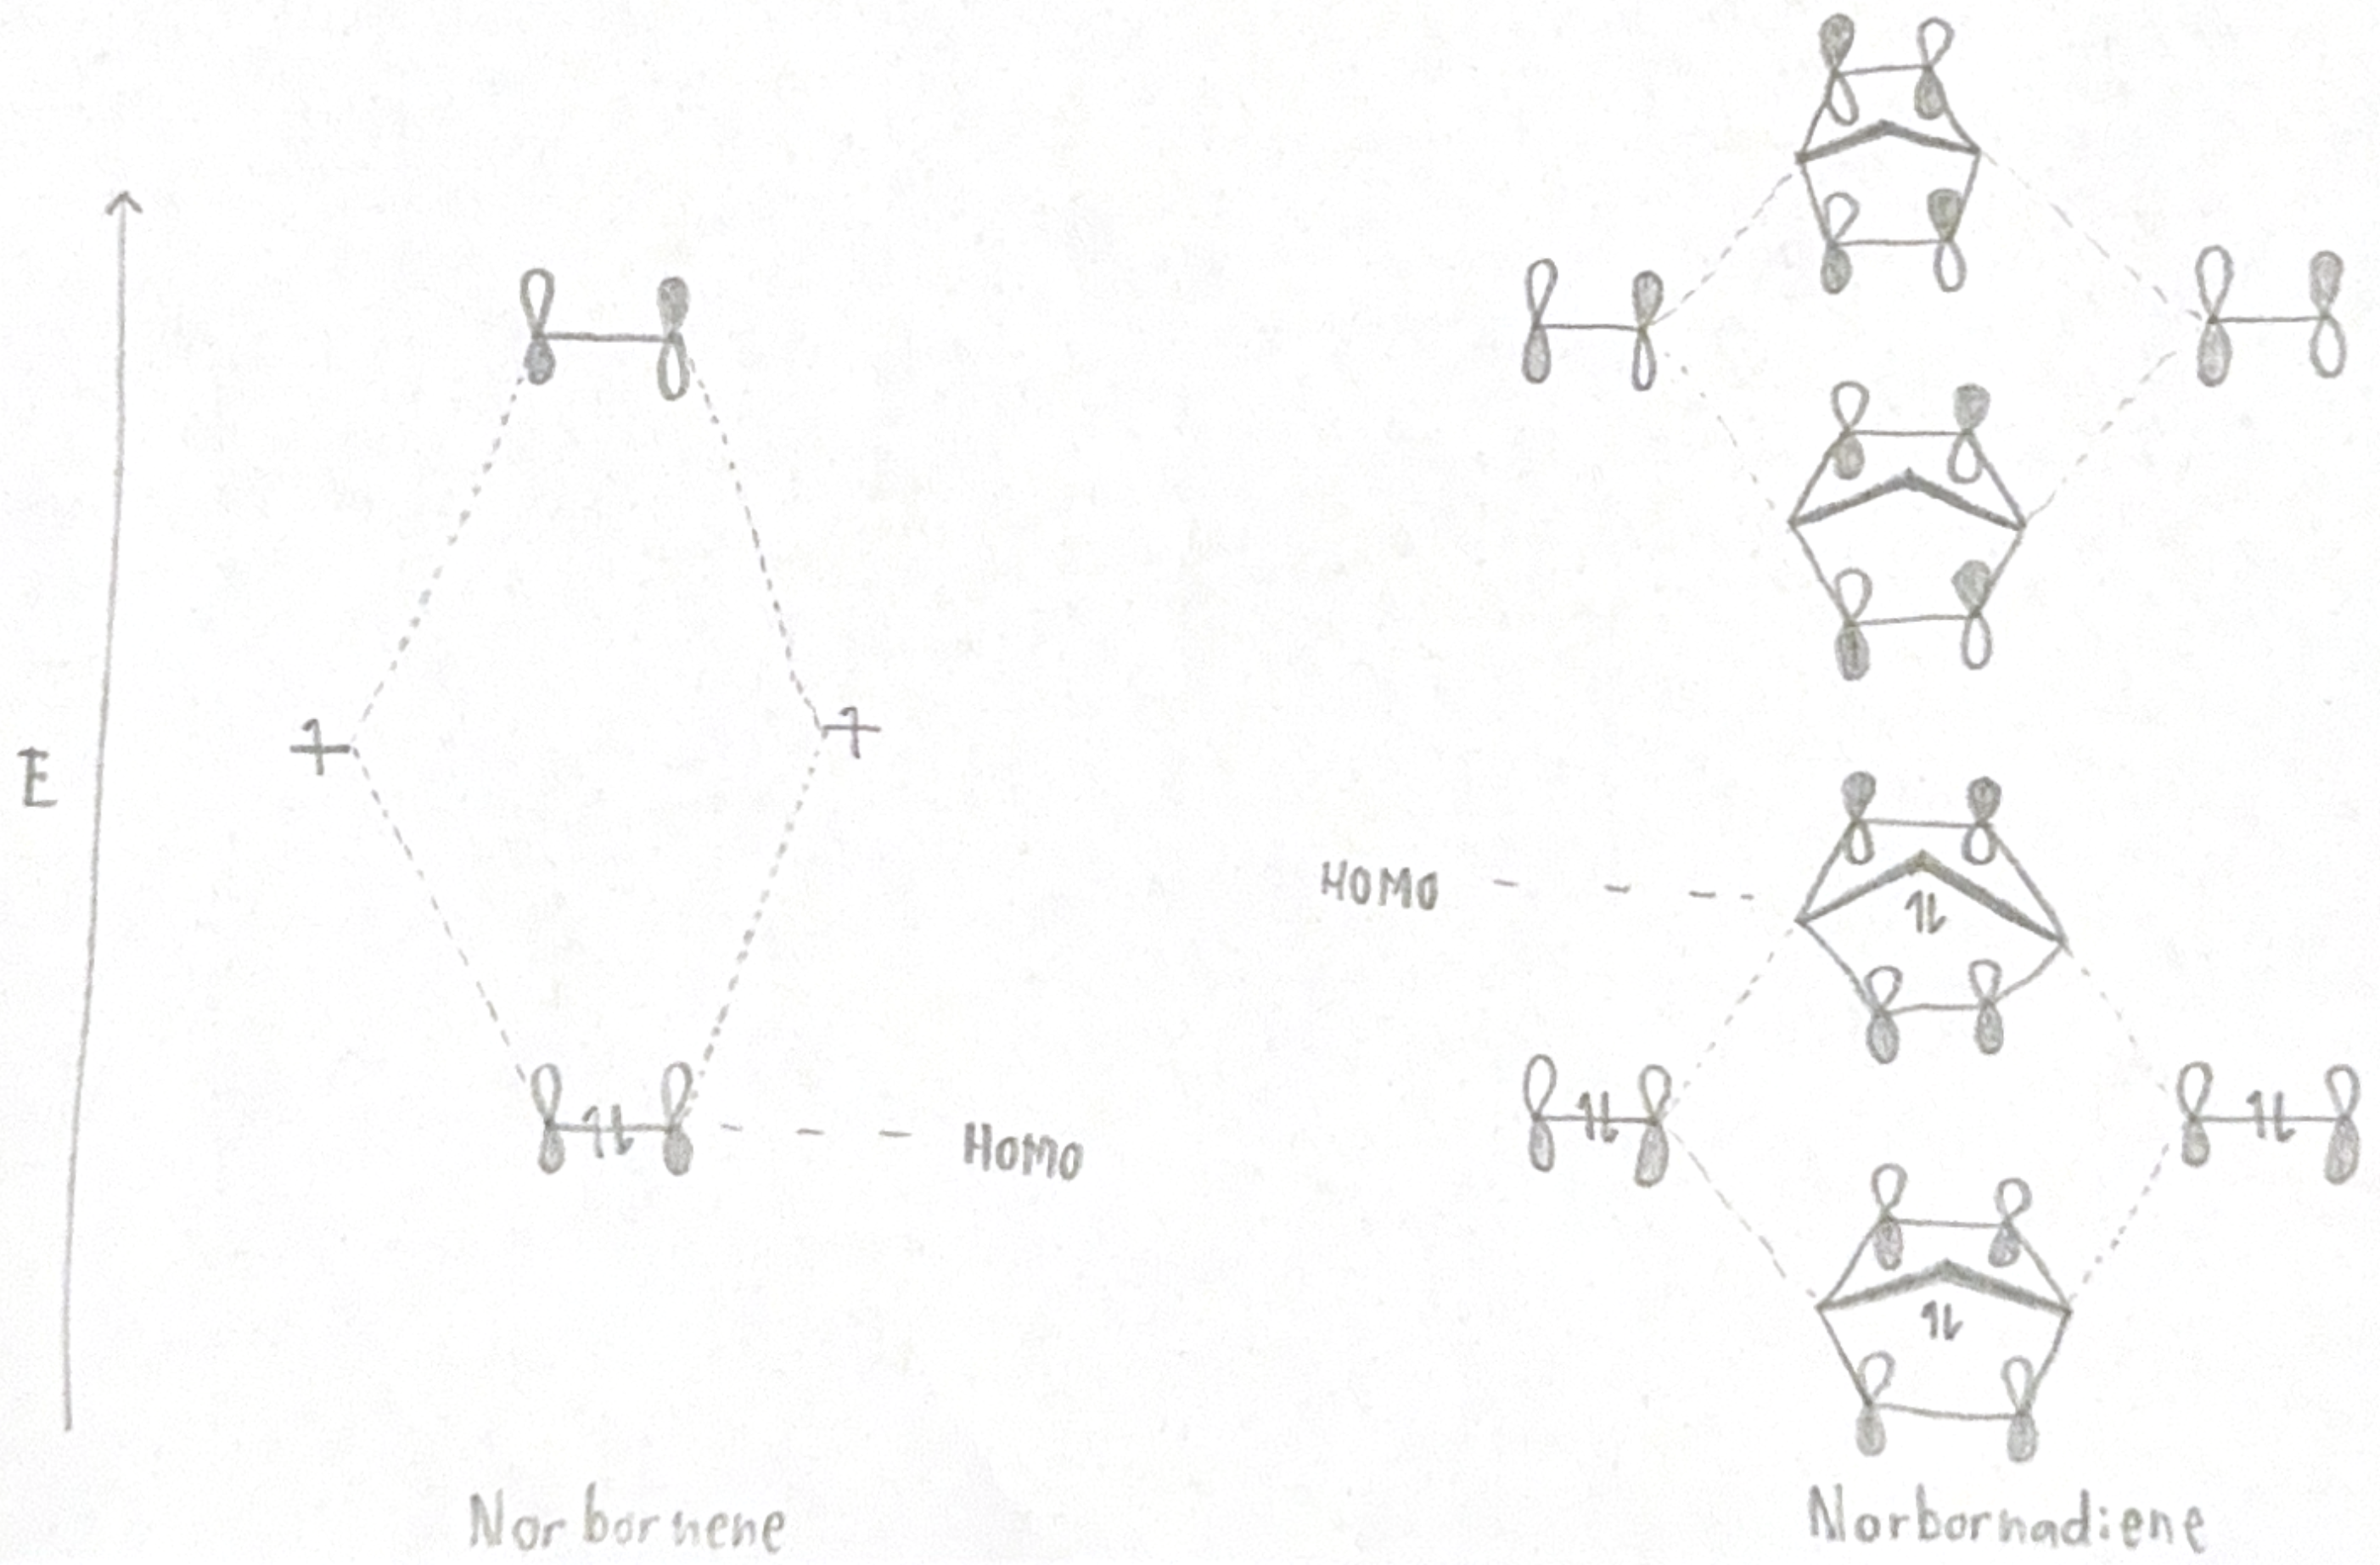
\includegraphics[width=0.9\linewidth]{PSet1Q4a.png}
            \end{center}
        \end{proof}
        \item Norbornadiene derivatives can be converted to quadricyclane derivatives under UV irradiation. Quadricyclanes are highly strained molecules, yet they are thermally stable.
        \begin{center}
            \includegraphics[width=0.4\linewidth]{PSet1F7.png}
        \end{center}
        Provide a frontier MO analysis\footnote{Per Jonathan's 9/24 Canvas announcement, we can use \emph{any} MO analysis discussed in lecture; in particular, we are not restricted to Fukui's FMO.} to explain why quadricyclane is thermally stable.
        \begin{proof}
            The reaction depicted above is a photochemical $[2+2]$ cycloaddition.\par
            To justify why the product is \emph{thermally} stable, let's correlate the product orbitals to the starting material orbitals. Note that in doing so, we will identify the symmetry of each molecular orbital by the two persistent symmetry operations, as suggested by \textcite[880]{bib:Anslyn}. Namely, we will look at the $\sigma$-plane discussed in class, and a perpendicular $\sigma_v$ plane running from left to right across the page. Note also that the remainder of the quadricyclane and norbornadiene rings outside of the 4-membered ring will be omitted from the following diagram for clarity.
            \begin{center}
                \includegraphics[width=0.9\linewidth]{PSet1Q4b.png}
            \end{center}
            As such, we can see that a thermal cycloreversion is forbidden/disfavored because it would involve creating a high-energy excited state of norbornadiene.
        \end{proof}
    \end{enumerate}
    \item Please use computational tools to complete this question. We will be using a browser-based quantum chemistry platform (\href{https://rowansci.com/}{Rowan}) for this course.
    \begin{enumerate}
        \item Create an account on Rowan (\url{https://rowansci.com/}) using your MIT email.
        \begin{itemize}
            \item To learn how to submit a job on Rowan, please watch this video tutorial: \url{https://docs.rowansci.com/web-interface/run-a-simple-job} and/or read this overview: \url{https://docs.rowansci.com/web-interface/submit/geometry-optimization}.
            \item More information on how to use Rowan (as well as additional tools) can be found here: \url{https://docs.rowansci.com/web-interface}.
        \end{itemize}
        \item Ethane (\ce{H3CCH3}).
        \begin{enumerate}
            \item Using any means, build a molecular model for ethane in Rowan. Then, perform a geometry optimization using the PBE0 functional and the def2-SVP basis set. Take a screenshot of the webpage before submitting the job and paste it here.
            \begin{itemize}
                \item Note: this job should not take more than 1 minute to run (not including queue time). If it takes significantly longer, consider adjusting your initial bond lengths/angles.
            \end{itemize}
            \begin{proof}
                {\color{white}hi}
                \begin{center}
                    \includegraphics[width=0.9\linewidth]{PSet1Q5bi.png}
                \end{center}
            \end{proof}
            \item Convert the optimized structure into Cartesian (XYZ) coordinates and paste them here.
            \begin{proof}
                {\color{white}hi}\\
                C       -0.75677857 -0.05411065 0.03565919\\
                C       0.75677857 0.05411065 -0.03565919\\
                H       -1.15393947 -0.71157723 -0.75360372\\
                H       -1.23964754 0.92846958 -0.08395828\\
                H       -1.08879565 -0.46588635 1.00165110\\
                H       1.08879566 0.46588615 -1.00165118\\
                H       1.15393946 0.71157739 0.75360359\\
                H       1.23964755 -0.92846954 0.08395849
            \end{proof}
            \item What is the calculated optimized \ce{C-C} bond distance? What is the \ce{H-C-H} bond angle(s)?\footnote{Per Jonathan's 9/24 Canvas announcement, provide at least 4 significant figures for bond lengths and angles. If you previously had issues obtaining these values from Rowan, please try again as the problem should be resolved now. If you are still unable to get 4 significant figures from Rowan, contact Jonathan.}
            \begin{proof}
                \ce{C-C} bond distance: \SI{1.519}{\angstrom}.\\
                \ce{H-C-H} bond angle: \ang{107.26}.
            \end{proof}
        \end{enumerate}
        \item Ethyl cation (\ce{H3CCH2+}).
        \begin{enumerate}
            \item Using any means, build a molecular model for the ethyl cation in Rowan. Then, perform a geometry optimization using the PBE0 functional and the def2-SVP basis set. Take a screenshot of the webpage before submitting the job and paste it here.
            \begin{itemize}
                \item Note: this job should not take more than 1 minute to run (not including queue time). If it takes significantly longer, consider adjusting your initial bond lengths/angles.
            \end{itemize}
            \begin{proof}
                {\color{white}hi}
                \begin{center}
                    \includegraphics[width=0.9\linewidth]{PSet1Q5ci.png}
                \end{center}
            \end{proof}
            \item Convert the optimized structure into Cartesian (XYZ) coordinates and paste them here.
            \begin{proof}
                {\color{white}hi}\\
                H       -1.22084801 0.85147887 0.51800484\\
                C       -0.64953900 -0.05423031 0.27448674\\
                H       -0.17606995 0.13377943 -0.93834042\\
                H       -1.18064873 -1.01496471 0.24418216\\
                C       0.70652007 0.01092307 0.02934683\\
                H       1.28037984 -0.89670040 -0.20069381\\
                H       1.24020579 0.96971405 0.07301367
            \end{proof}
            \item What is the calculated optimized \ce{C-C} bond distance? What is the \ce{H-C-H} bond angle(s)?
            \begin{proof}
                \ce{C-C} bond distance: \SI{1.380}{\angstrom}.\\
                \ce{H-C-H} bond angle: \ang{118.43} and \ang{105.89}.
            \end{proof}
        \end{enumerate}
        \item Now, using qualitative MO arguments based on your calculations, discuss at least two factors contributing to the differing \ce{C-C} bond lengths in ethane vs ethyl cation.
        \begin{proof}
            Due to hyperconjugation, there is donation from the adjacent \ce{C-H} $\sigma$-bond into the carbocation's empty $p$-orbital that forms a 3c-2e bond. This donation increases the bond order of the \ce{C-C} bond, shortening it compared to ethane. Additionally, the $sp^2$-like bond angles means --- per the hybridization index --- that the hybrid orbitals have more $s$-character and hence will be shorter.
        \end{proof}
    \end{enumerate}
\end{enumerate}




\end{document}